\documentclass[aspectratio=169]{beamer}
\usetheme{Madrid}
\usepackage[utf8]{inputenc}
\usepackage{graphicx}
\graphicspath{{./figures/}}
\usepackage{amsmath}
\usepackage{booktabs}
\usepackage{hyperref}
\usepackage[
  style=nejm, 
  citestyle=numeric-comp,
  sorting=none
]{biblatex}
\addbibresource{sample.bib}

\title[Analisis H1N1 1918]{Analisis Parameter Transmisi Epidemi Influenza H1N1 1918 di Baltimore: Estimasi \texorpdfstring{$R_0$}{R0}, \texorpdfstring{$R_c$}{Rc}, dan \texorpdfstring{$R_t$}{Rt}}
\author[Hanafi dkk.]{Ammar Hanafi \and Fariz Naufal Gustoro \and Rahmat Affandi \and Yohanes Nathael \and Zavier Raiyan Dana}
\institute[UI]{Departemen Matematika, Universitas Indonesia, Depok, Indonesia.}
\date{}

\begin{document}

\begin{frame}
    \titlepage
\end{frame}

\begin{frame}{Latar Belakang}
    \begin{itemize}
        \item Pandemi Influenza tahun 1918 merupakan wabah historis ekstrem yang melanda berbagai kawasan, termasuk Baltimore.
        \item Kerangka pemodelan metrik angka reproduktif ($R_0$, $R_c$, $R_t$) dibutuhkan untuk mengukur cepatnya transmisi penyakit.
        \item Pengukuran tunggal $R_0$ tidak dapat menangkap dinamika perubahan akibat intervensi (\textit{Non-Pharmaceutical Interventions/NPI}).
        \item \textbf{Tujuan studi:} 
        \begin{itemize}
            \item Mengestimasi besaran $R_0$ menggunakan eksponensial Euler-Lotka.
            \item Mensimulasikan probabilitas persebaran $R_c$ (Wallinga \& Teunis) dan sebaran dinamis $R_t$ (Cori \textit{et al.}).
            \item Membandingkan reduksi ambang penularan terhadap NPI di Baltimore.
        \end{itemize}
    \end{itemize}
\end{frame}

\begin{frame}{Angka Reproduktif dan Parameter H1N1}
    \begin{itemize}
        \item \textbf{Angka Reproduksi Dasar ($R_0$):} Rata-rata infeksi sekunder di awal wabah. Berkorelasi linier dengan laju kemunculan eksponensial $r$.
        \item \textbf{Persamaan Euler-Lotka:} Pendekatan turunan \textit{Moment Generating Function(MGF)} yang dimodifikasi terhadap sumbu \textit{generation time}.
        \item \textbf{Interval Generasi H1N1:} Distribusi waktu transisi diasumsikan sebagai sebaran \textbf{Gamma} dengan rerata $\mu \approx 2,6$ hari dan simpangan $\sigma \approx 1,5$ hari berdasarkan studi \cite{White2009}.
        \item \textbf{Estimasi Transisi:}
        \begin{itemize}
            \item \textbf{$R_c$} (Metode Wallinga-Teunis): \textit{Cohort} laju estimasi sekunder di masa depan (perspektif \textit{forward}).
            \item \textbf{$R_t$} (Metode Cori \textit{et al.}): \textit{Instantaneous} laju berdasarkan agregat interaksi masa berjalan (perspektif \textit{sliding window}).
        \end{itemize}
    \end{itemize}
\end{frame}

\begin{frame}{Eksplorasi Kasus Insidensi}
    \begin{columns}
        \begin{column}{0.5\textwidth}
            \begin{figure}
                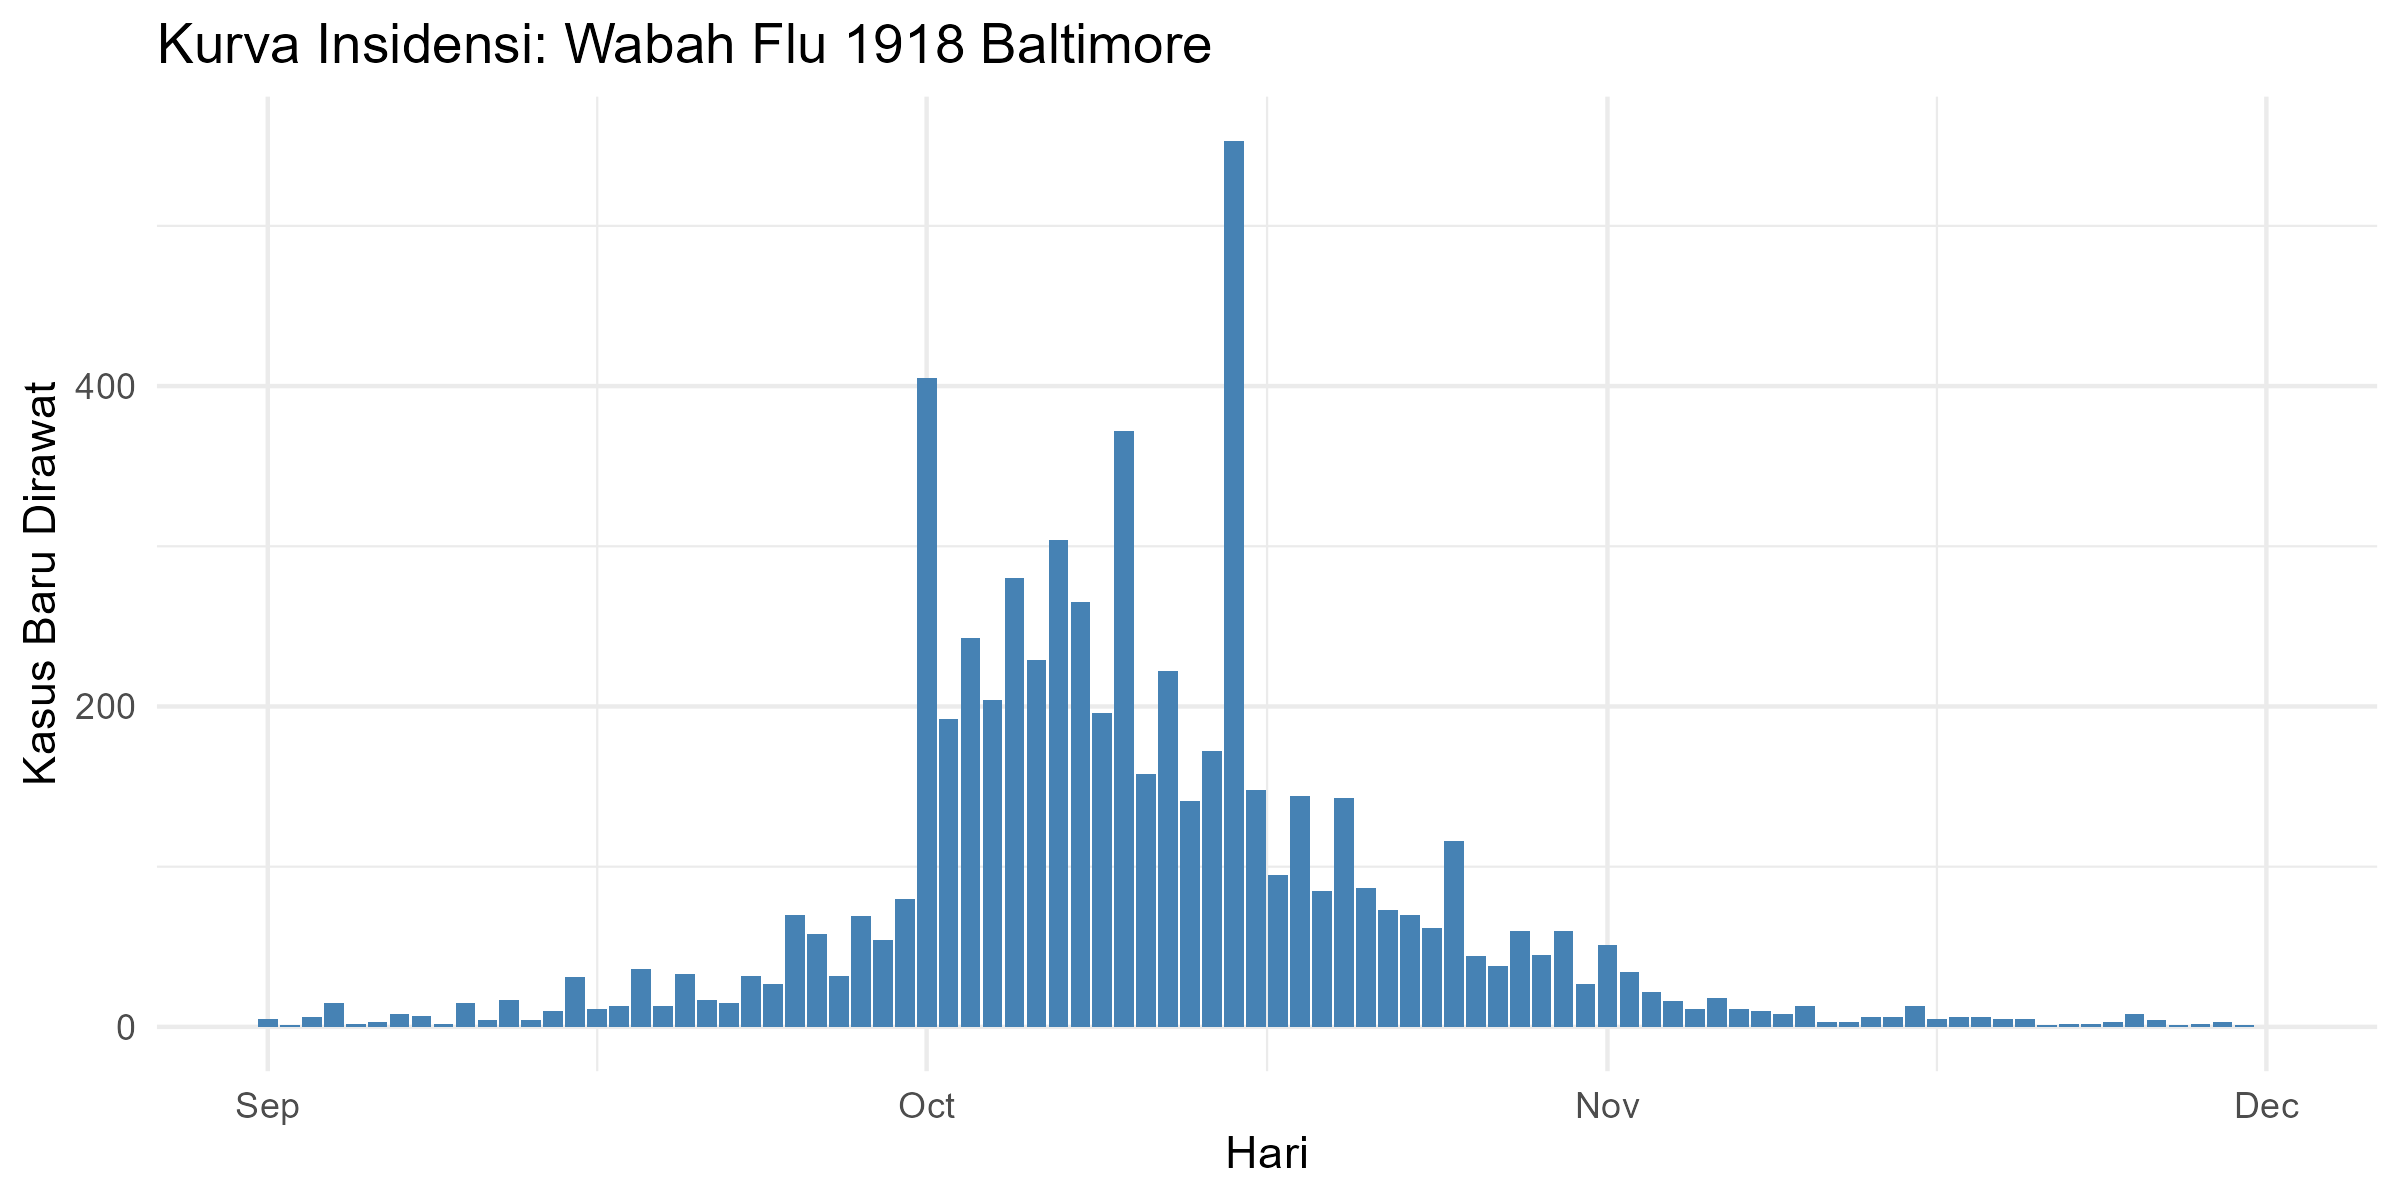
\includegraphics[width=\textwidth,height=0.6\textheight,keepaspectratio]{kurva_insidensi.png}
                \caption{Kurva Kasus H1N1}
            \end{figure}
        \end{column}
        \begin{column}{0.5\textwidth}
            \begin{itemize}
                \item Paket dataset \texttt{Flu1918} memberikan distribusi lonjakan perhari \textit{incident}.
                \item Eskalasi sangat drastis dan agresif mendestruksi populasi rentan (\textit{susceptible}) di Baltimore.
                \item Kepadatan gelombang merepresentasikan beban maksimum bagi fasilitas dan manajemen karantina di kala itu.
            \end{itemize}
        \end{column}
    \end{columns}
\end{frame}

\begin{frame}{Hasil Estimasi $R_0$ (Euler-Lotka)}
    \begin{itemize}
        \item Fase pelandaian hari ke-10 hingga 16 menunjukkan tren sebaran eksponensial.
        \item Laju pertumbuhan diregresi dengan Model \textit{Poisson} ($GLM$):
        \begin{equation}
           \text{Laju Eksponensial } (r) \approx 0,096 \text{ infeksi / hari}
        \end{equation}
        \item Konversi menggunakan relasi log-Gamma Euler-Lotka, dengan $k = (\mu/\sigma)^2 \approx 3,00$ dan $\theta = \sigma^2/\mu \approx 0,865$:
        \begin{equation}
            R_0 = (1 + r \theta)^k = (1 + (0,096 \times 0,865))^3 \approx 1,27
        \end{equation}
        \item Skala $R_0 \approx 1,27$ mendefinisikan patogenisitas medium di ekosistem urban sebelum isolasi paksa diberlakukan.
    \end{itemize}
\end{frame}

\begin{frame}{Estimasi Cohort Reproduction ($R_c$)}
    \begin{columns}
        \begin{column}{0.5\textwidth}
            \begin{figure}
                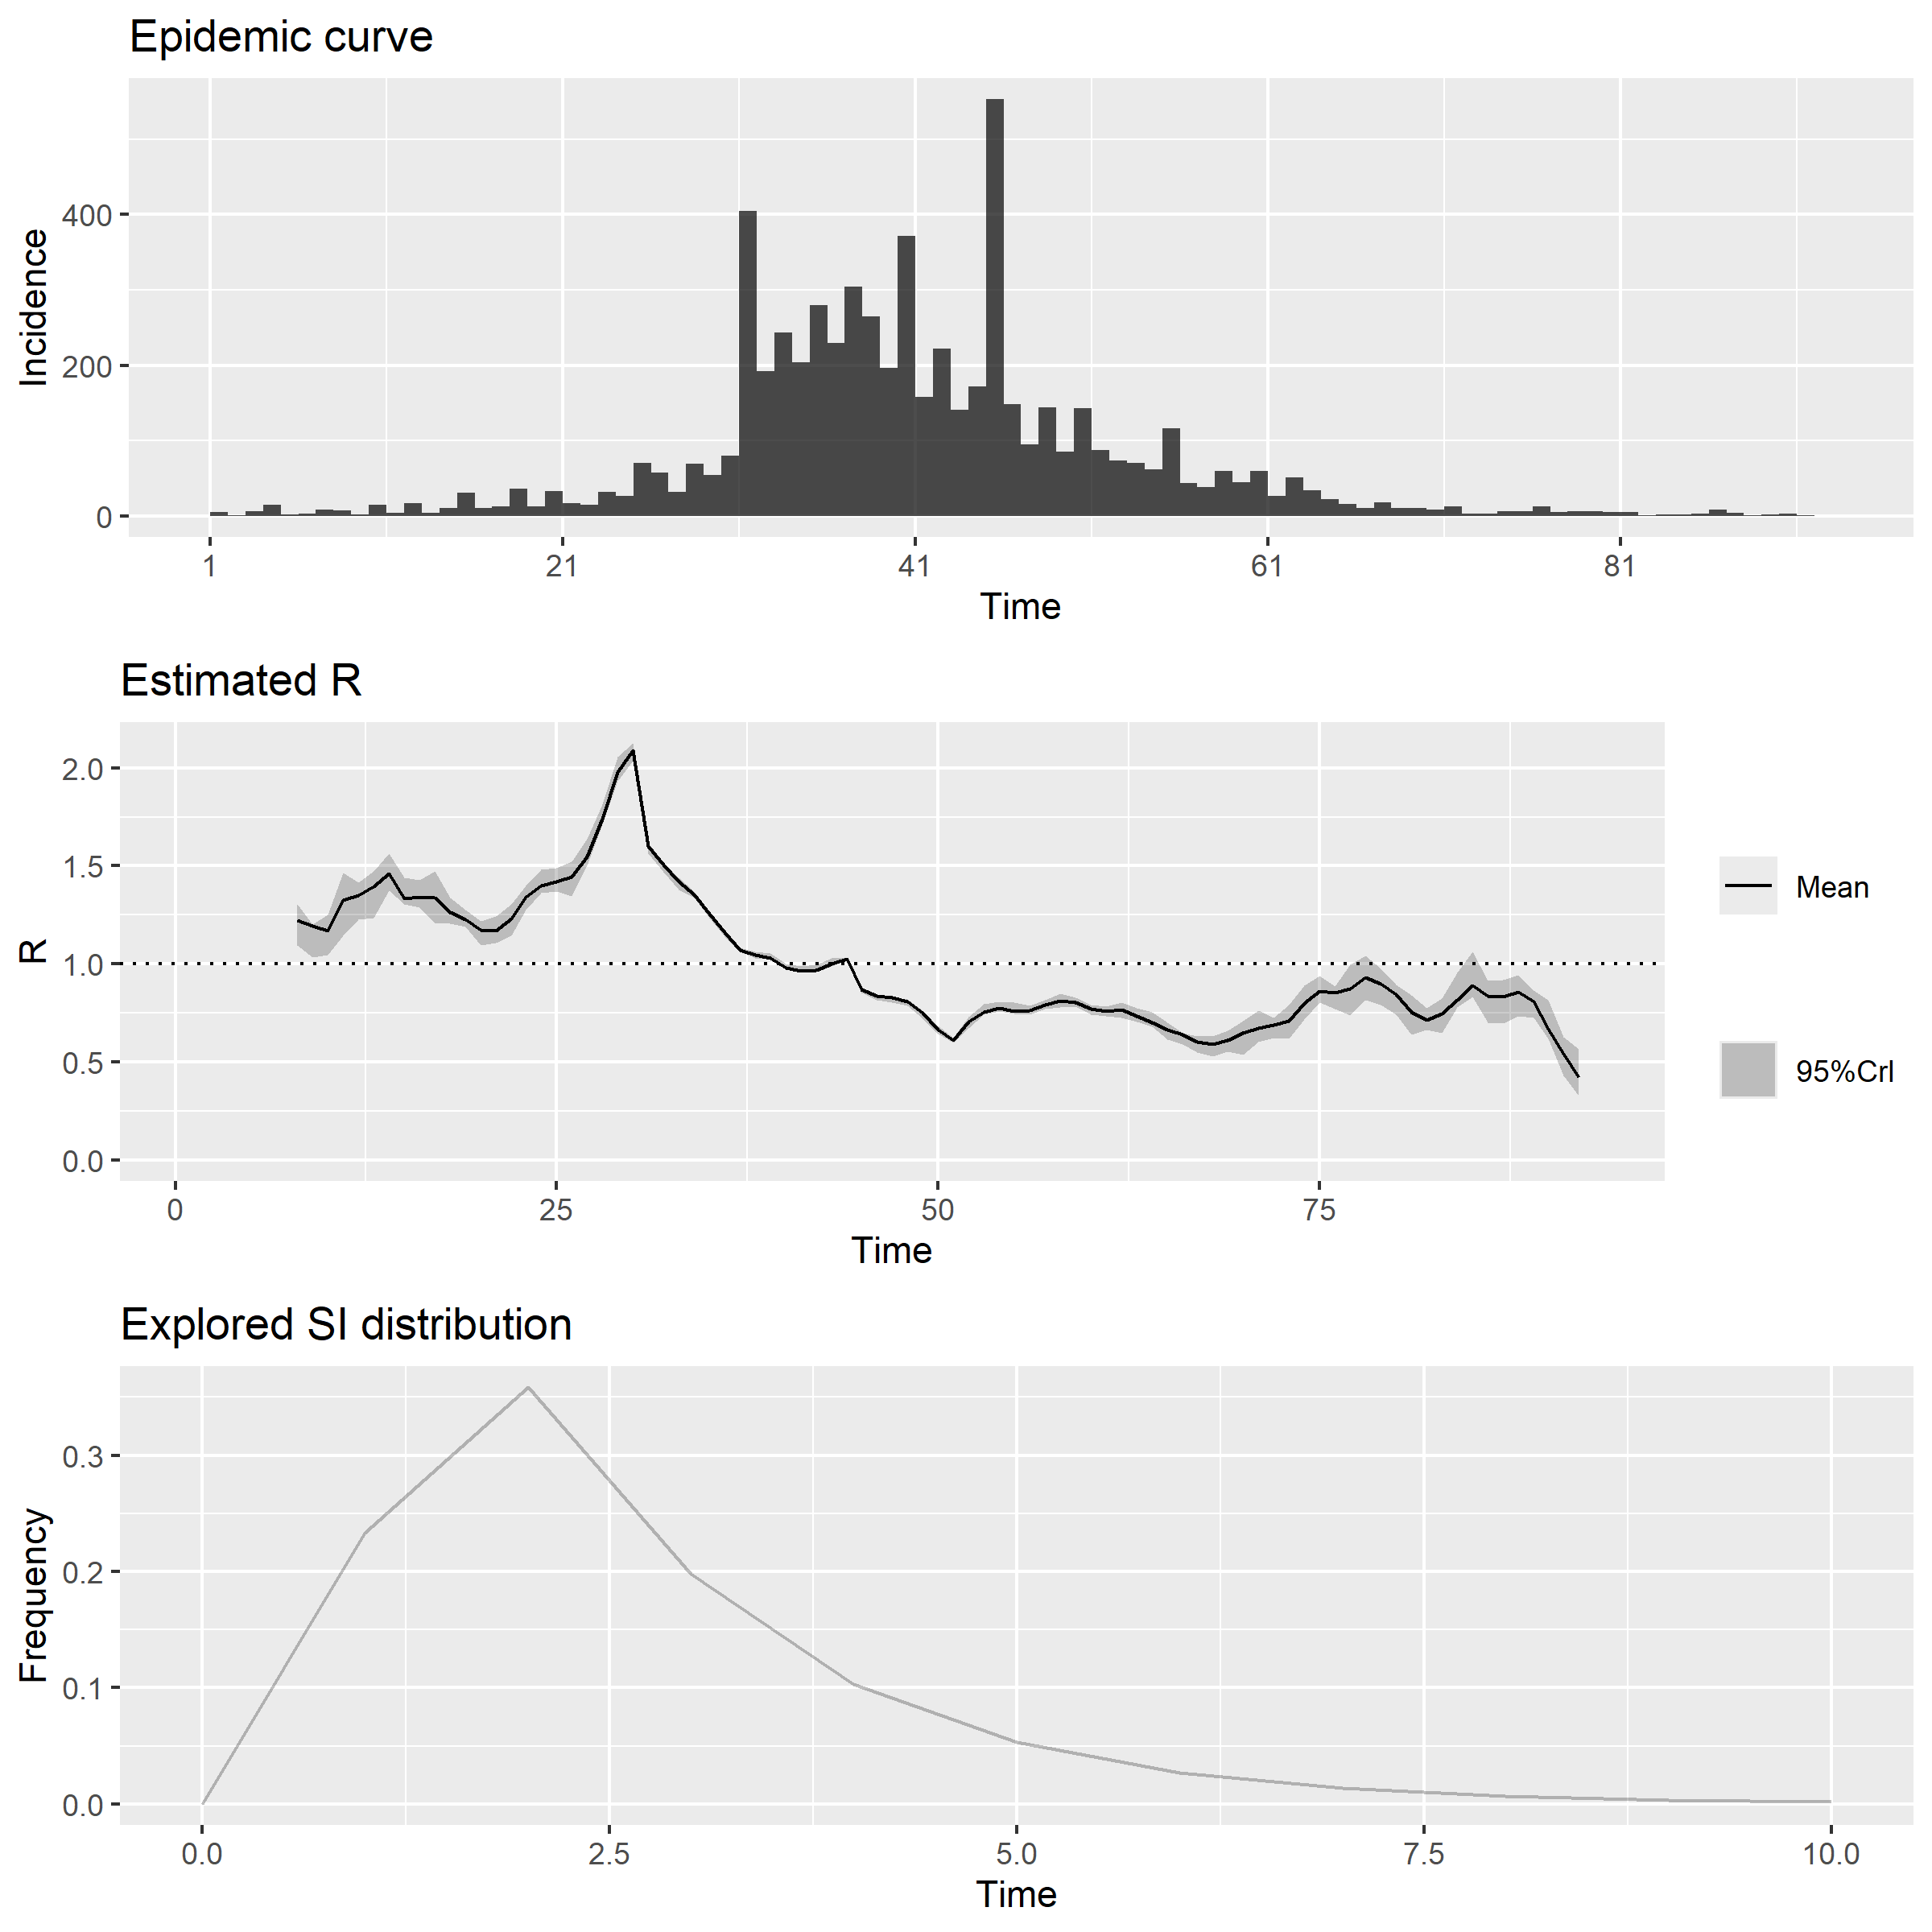
\includegraphics[width=\textwidth,height=0.6\textheight,keepaspectratio]{plot_rc.png}
                \caption{Metrik $R_c$ (Wallinga-Teunis)}
            \end{figure}
        \end{column}
        \begin{column}{0.5\textwidth}
            \begin{itemize}
                \item $R_c$ bergelembung tajam di minggu awal.
                \item Responsivitas kurva \textit{Cohort} menunjukkan individu sukses mendedahkan rantai transmisi sebelum meredup.
                \item Indikasi kelelahan wabah terihat dari kemerosotan instan nilai $R_c$ di ujung fase jenuh.
            \end{itemize}
        \end{column}
    \end{columns}
\end{frame}

\begin{frame}{Estimasi Instantaneous Reproduction ($R_t$)}
    \begin{columns}
        \begin{column}{0.5\textwidth}
            \begin{figure}
                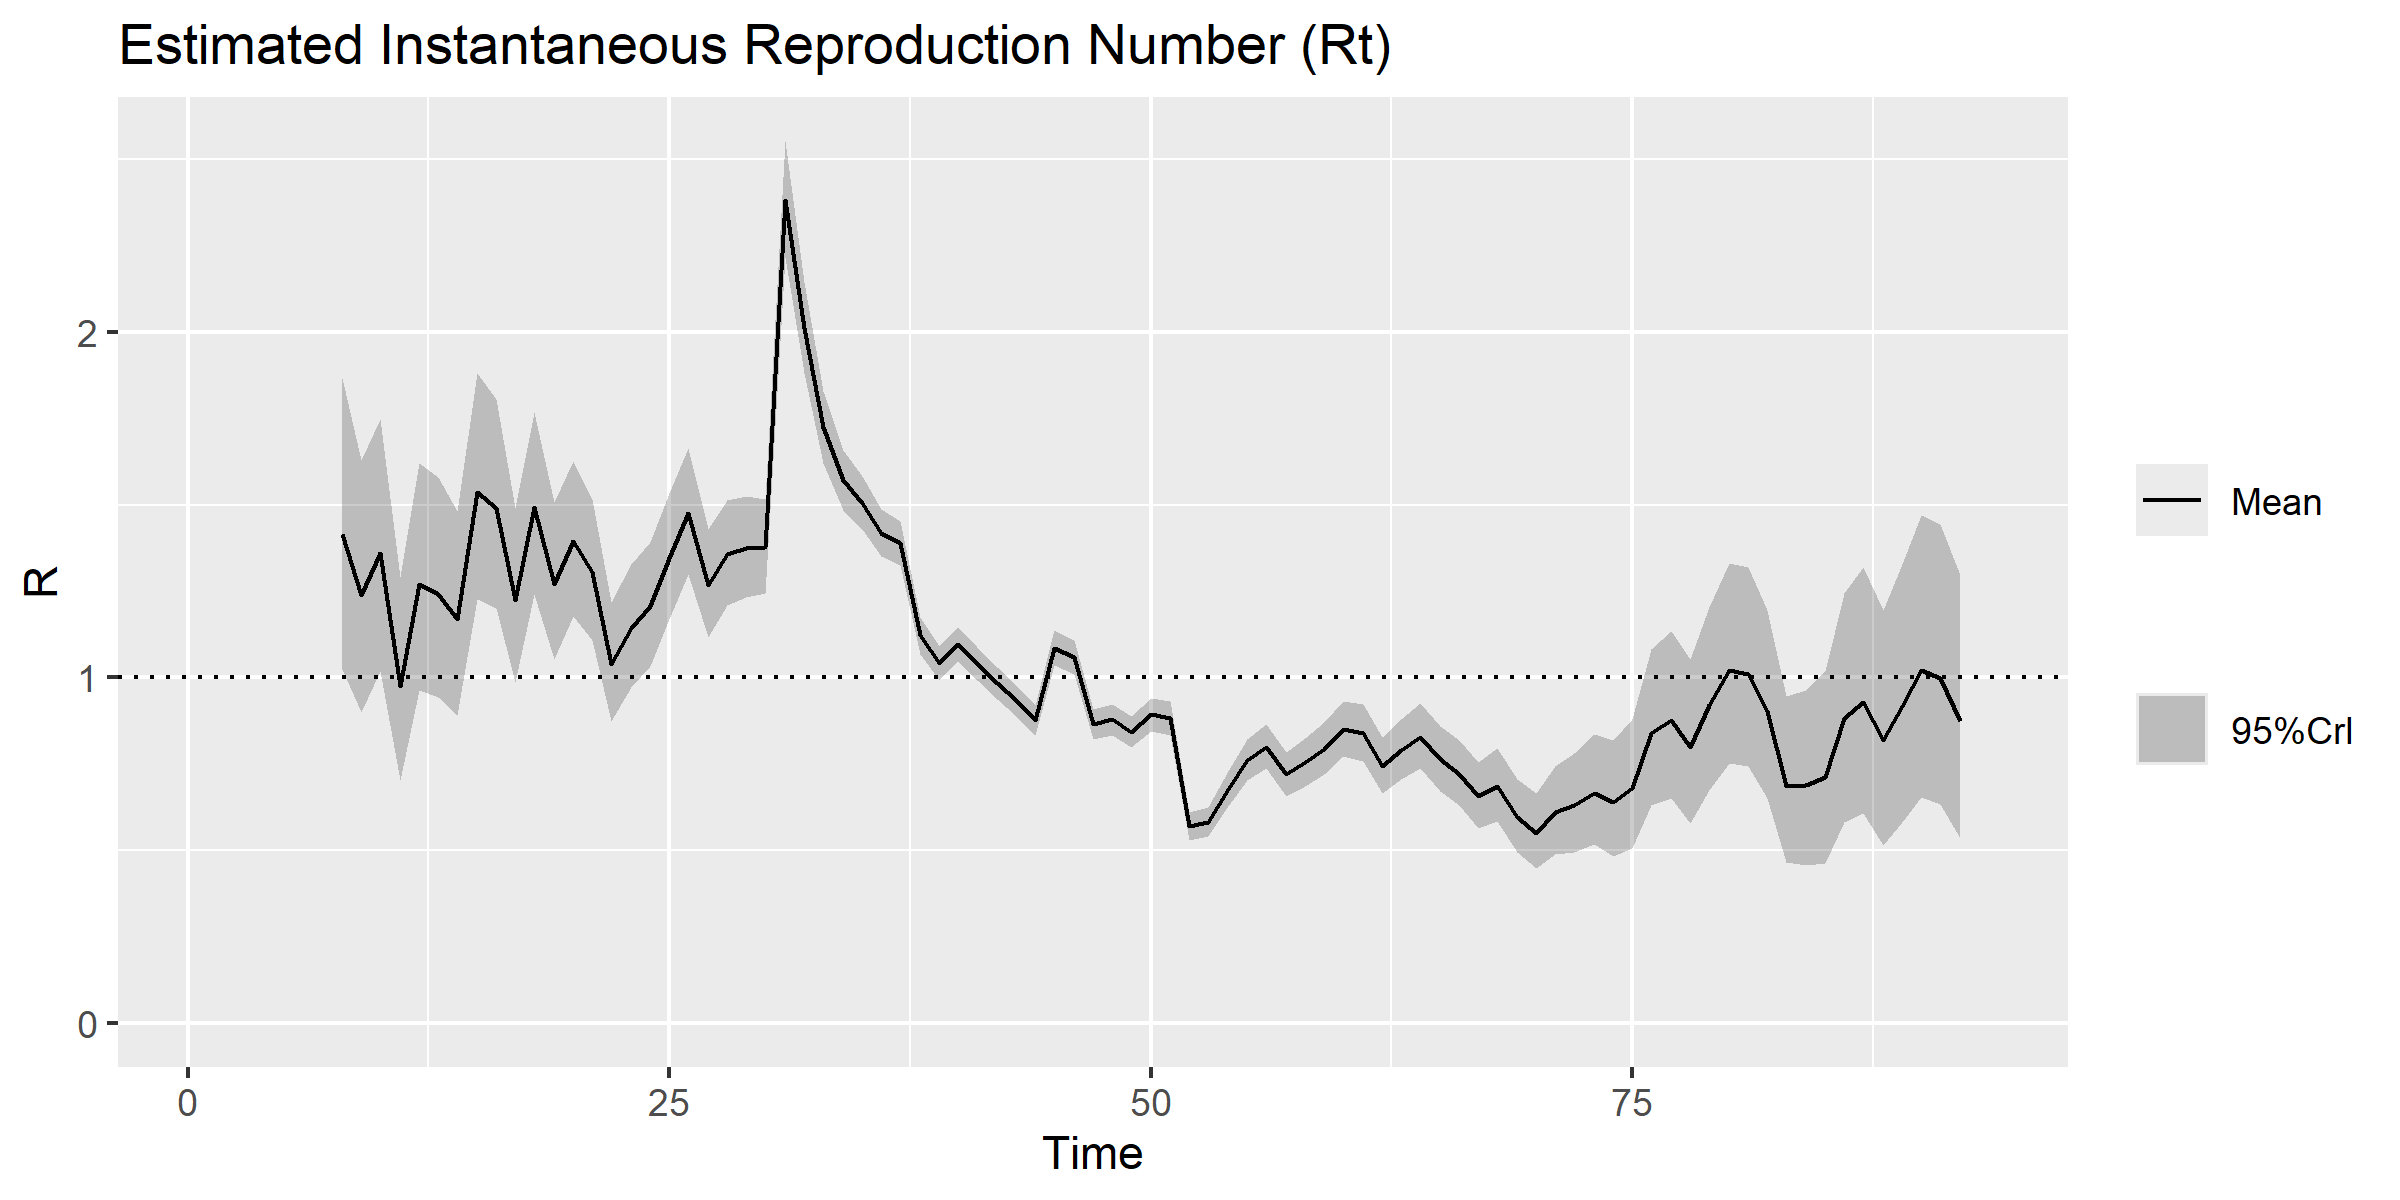
\includegraphics[width=\textwidth,height=0.6\textheight,keepaspectratio]{plot_rt.png}
                \caption{Metrik $R_t$ dengan Jendela Cori \textit{et al.}}
            \end{figure}
        \end{column}
        \begin{column}{0.5\textwidth}
            \begin{itemize}
                \item Menyamakan respons seketika NPI terhadap fluktuasi grafik berjalan.
                \item Angka median tertahan dan berangsur turun.
                \item Berdasarkan kerangka data estimasi, pelemahan kurva menembus secara konsisten di bawah ambang statis $R_t \leq 0,99$ \textbf{terjadi pada Hari ke-42}.
            \end{itemize}
        \end{column}
    \end{columns}
\end{frame}

\begin{frame}{Diskusi Kausalitas Transmisi}
    \begin{itemize}
        \item \textbf{Pergeseran Phase-Lag:} Kurva $R_c$ (cohort) melemah drastis lebih awal dibandingkan $R_t$. Hal ini ditimbulkan fenomena \textit{shift}: pelacakan berbasis kohort menimbang subyek hari ini sudah gagal menularkan siapa pun ke depannya (\textit{forward parameter}). Sedangkan pada estimasi $R_t$, perhitungan masa agregat infeksi yang menderet menjadikan rekam riwayat ikut mendominasi \textit{lag} penyusutan transmisi.
        \item \textbf{Efektifitas NPI:} Kesetimbangan $\leq 1,00$ yang kokoh pasca sebulan bertepatan dengan instruksi preskriptif Dewan Kesehatan Maryland:
        \begin{itemize}
            \item Penertiban kegiatan \textit{ban on mass gathering}.
            \item Restriksi fasilitas persekolahan dan teater.
            \item Penguatan isolasi penderita di tengah menipisnya kompartemen Inang Naif (\textit{Depletion of Susceptible Herd}).
        \end{itemize}
    \end{itemize}
\end{frame}

\begin{frame}{Kesimpulan}
    \begin{itemize}
        \item Pemodelan analitis gelombang H1N1 pada kasus Baltimore membuktikan Angka Reproduksi setingkat penyebaran \textbf{medium severity} ($R_0 \approx 1,27$).
        \item Intervensi non-farmasi sukses mengerem laju penyebaran sehingga menembus ambang $R_t < 1,0$ secara kuat dari evaluasi empiris pada kisaran \textbf{Hari ke-42}.
        \item Varian metrik analitis (Euler, Cohort dan Jendela probabilistik) penting digunakan bersama-sama karena metrik statik saja gagal mempertimbangkan \textit{time-lag} imunitas dari NPI.
    \end{itemize}
\end{frame}

\begin{frame}[allowframebreaks]{Daftar Pustaka}
    \printbibliography
\end{frame}

\begin{frame}{Lampiran Kode}
    \begin{itemize}
        \item \textbf{Source Code Utama R (Eksplorasi Penuh ABC, Gillespie, dan MLE)} dapat diakses secara penuh memalui tautan resmi pengerjaan proyek g-drive berikut ini:\\
        \vspace{0.5cm}
        \href{https://drive.google.com/drive/folders/1DqDRFNOHEabSOpNSRC6R-MKyvHeqKuEu?usp=sharing}{\color{blue}{\underline{Tautan Ke Akses Source Code (GDRIVE)}}}
    \end{itemize}
\end{frame}

\end{document}
